% ============================================
% SECTION 2: Methodology
% ============================================
\section{Metodologia}

\begin{frame}{LA-CDIP Dataset - Construção}
\begin{columns}
\column{0.5\textwidth}
\textbf{Motivação:}
\begin{itemize}
    \item RVL-CDIP inadequado para ZSL
    \item Classes definidas por propósito
    \item Múltiplos subclasses por classe
\end{itemize}

\textbf{Solução - LA-CDIP:}
\begin{itemize}
    \item Foco em padrões estruturais
    \item Reorganização do RVL-CDIP
    \item Classes baseadas em layout visual
\end{itemize}

\column{0.5\textwidth}
\includegraphics[width=\textwidth]{images/class_comparison1.png}
\vspace{0.2cm}
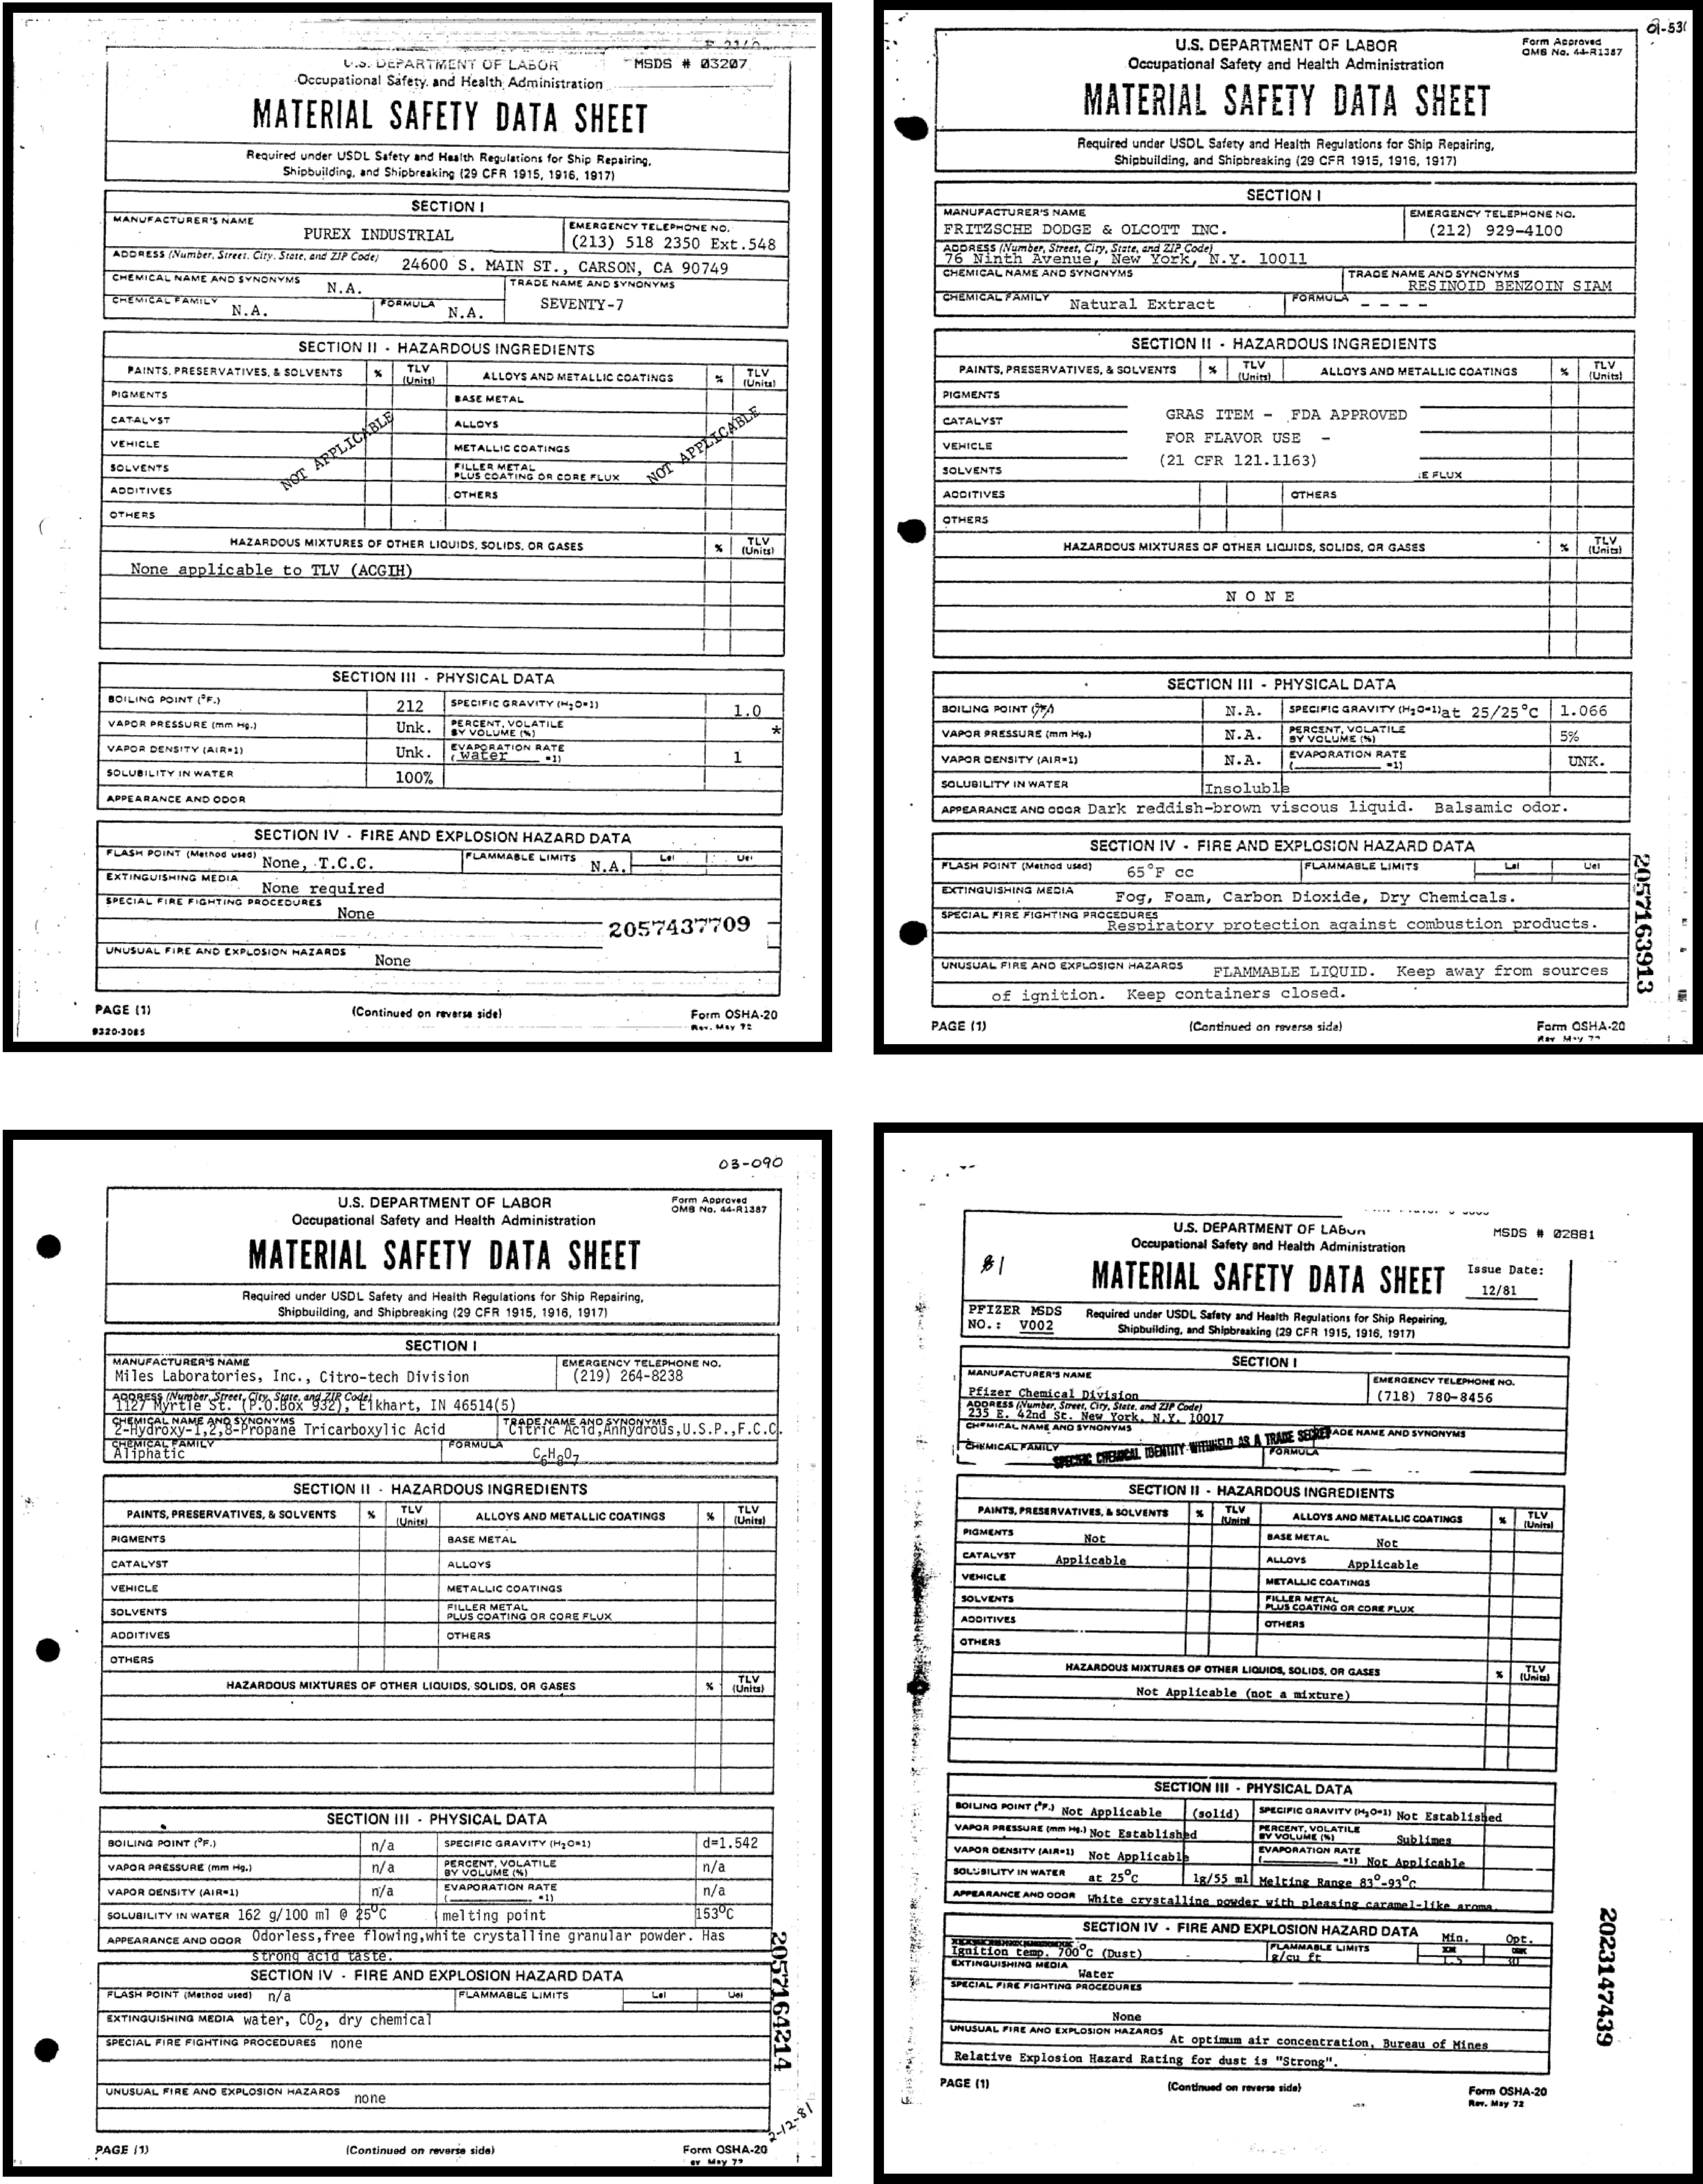
\includegraphics[width=\textwidth]{images/class_comparison2.png}
\end{columns}
\end{frame}

\begin{frame}{LA-CDIP Dataset - Processo de Labeling}
\begin{block}{Framework de Active Learning}
\textbf{Etapa 1: Clustering Preliminar}
\begin{itemize}
    \item Modelo privado de metric learning
    \item Hierarchical Agglomerative Clustering com estratégia de Ward
    \item Número dinâmico de clusters
\end{itemize}

\textbf{Etapa 2: Reorganização Manual}
\begin{itemize}
    \item Limpeza dos clusters (um padrão por cluster)
    \item Merge de clusters com padrões similares
    \item Validação independente para consistência intra e inter-classe
\end{itemize}
\end{block}
\end{frame}

\begin{frame}{Visual Document Matching - Arquitetura}
\begin{columns}
\column{0.6\textwidth}
\textbf{Abordagem:}
\begin{itemize}
    \item Siamese Networks
    \item Metric Learning
    \item Mapeamento para espaço de features
\end{itemize}

\textbf{Backbones Testados:}
\begin{itemize}
    \item ResNet (18, 34, 50, 101, 152)
    \item EfficientNet (B0-B3)
    \item MobileNetV3 (Small, Large)
    \item VGG (11, 13, 16, 19)
    \item Vision Transformer (Base, Large)
\end{itemize}

\column{0.4\textwidth}
\textbf{Princípio:}
\begin{center}
Documentos similares\\
$\downarrow$\\
Pequena distância\\
no espaço de features\\
\vspace{0.3cm}
Documentos diferentes\\
$\downarrow$\\
Grande distância\\
no espaço de features
\end{center}
\end{columns}
\end{frame}

\begin{frame}{Visual Document Matching - Ilustração}
\begin{center}
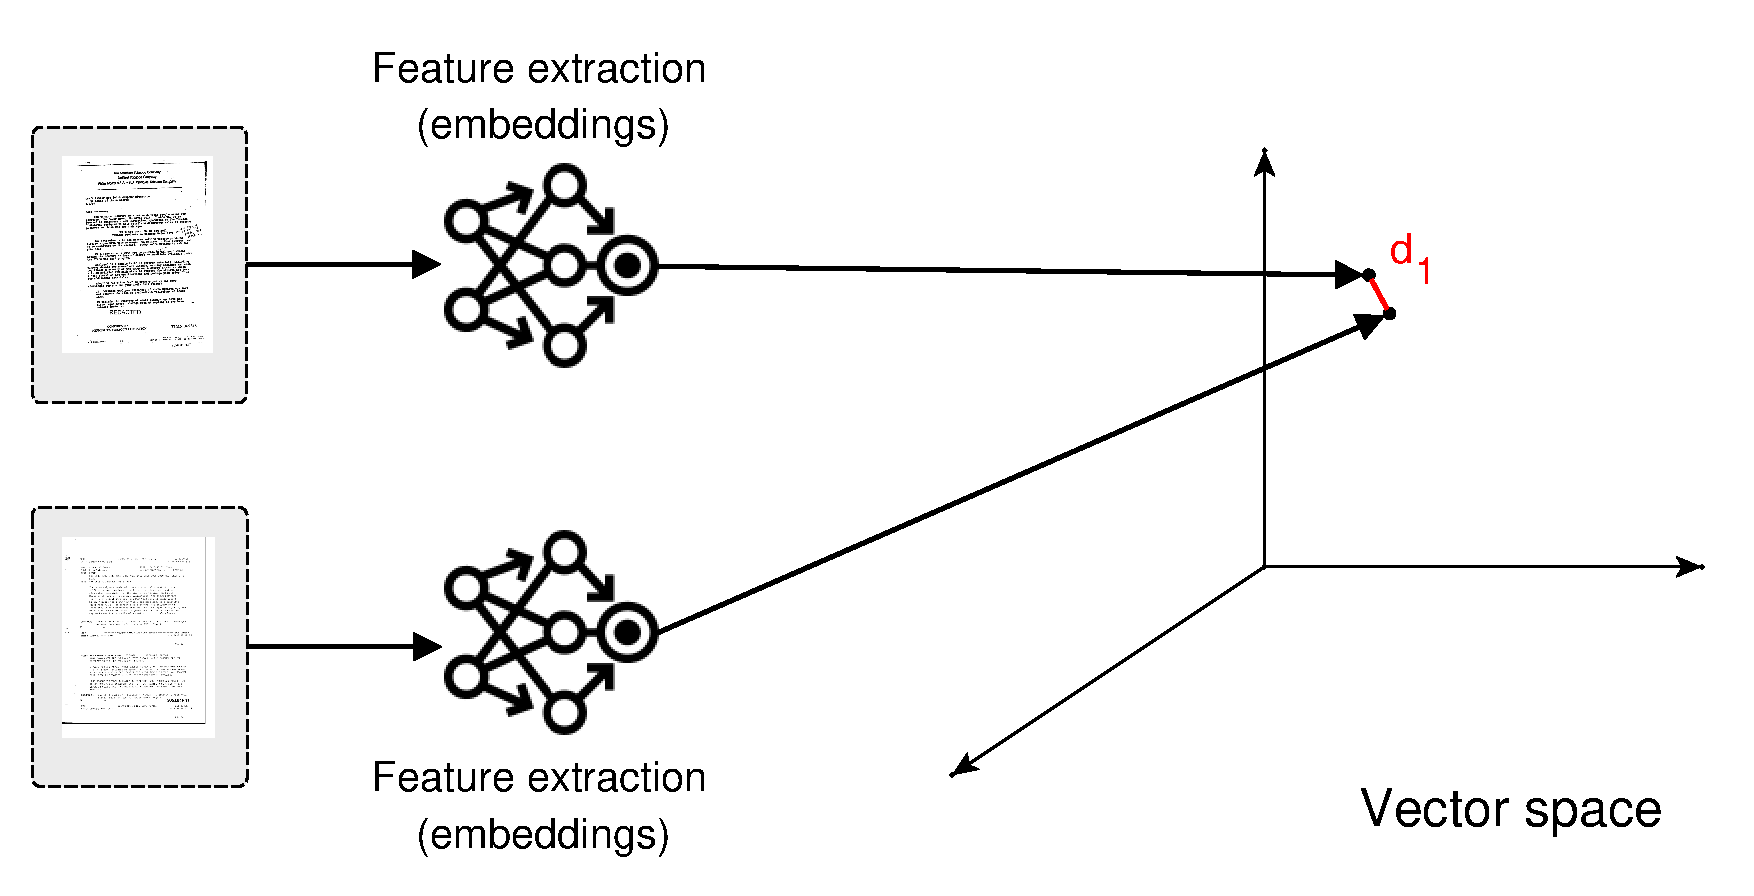
\includegraphics[width=0.8\textwidth]{images/vector_space_1.pdf}
\vspace{0.3cm}
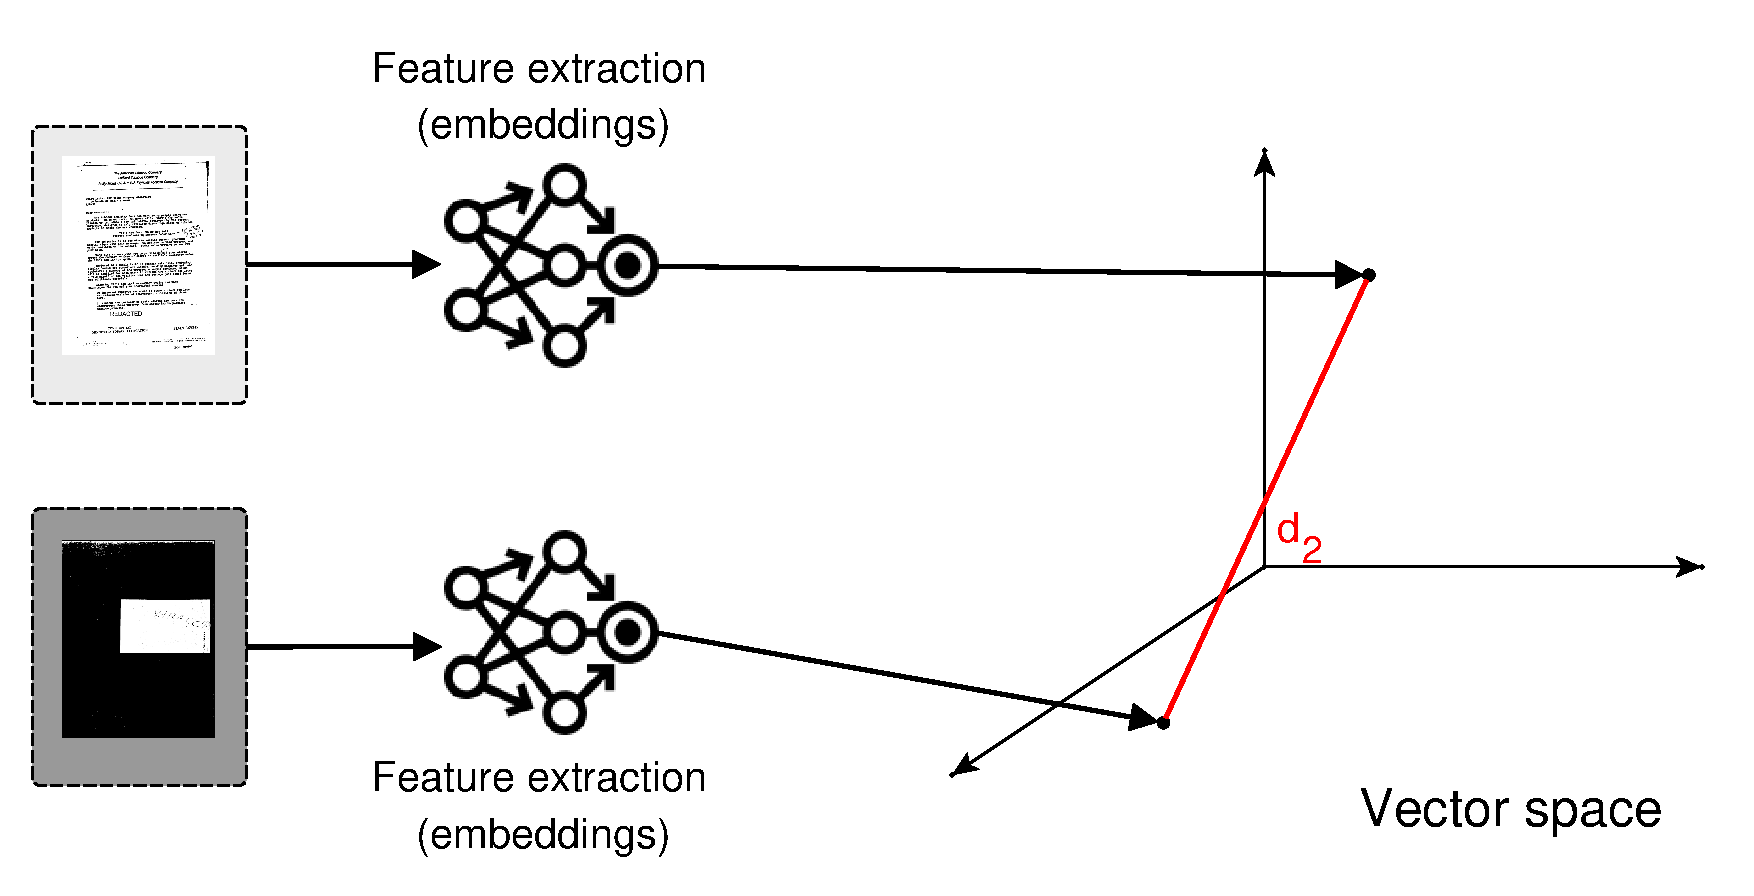
\includegraphics[width=0.8\textwidth]{images/vector_space_2.pdf}
\end{center}
\end{frame}

\begin{frame}{Pipeline de Treinamento}
\begin{block}{Configuração}
\begin{itemize}
    \item \textbf{Input:} Matriz RGB da imagem do documento
    \item \textbf{Pré-processamento:}
    \begin{itemize}
        \item Resize para (224, 224) para maioria dos modelos
        \item Normalização de 0--255 para 0--1
        \item Normalização com média e desvio padrão do split de treino
    \end{itemize}
    \item \textbf{Treinamento:}
    \begin{itemize}
        \item Formação de pares aleatórios
        \item Mesma probabilidade para todas as classes
        \item Contrastive Loss
        \item Sem data augmentation ou pair mining
    \end{itemize}
\end{itemize}
\end{block}
\end{frame}

\begin{frame}{Benchmarking com LLMs}
\begin{columns}
\column{0.5\textwidth}
\textbf{Modelos Avaliados:}
\begin{itemize}
    \item LLaVA 3.2 Vision
    \item InternVL 2.5
    \item Qwen2.5-VL
    \item GPT-4o (2024-11-20)
    \item GPT-4o-mini (2024-07-18)
\end{itemize}

\textbf{Avaliação:}
\begin{itemize}
    \item Zero-shot (sem fine-tuning)
    \item Pontuação de similaridade 0--100
    \item 5 níveis de categorização
\end{itemize}

\column{0.5\textwidth}
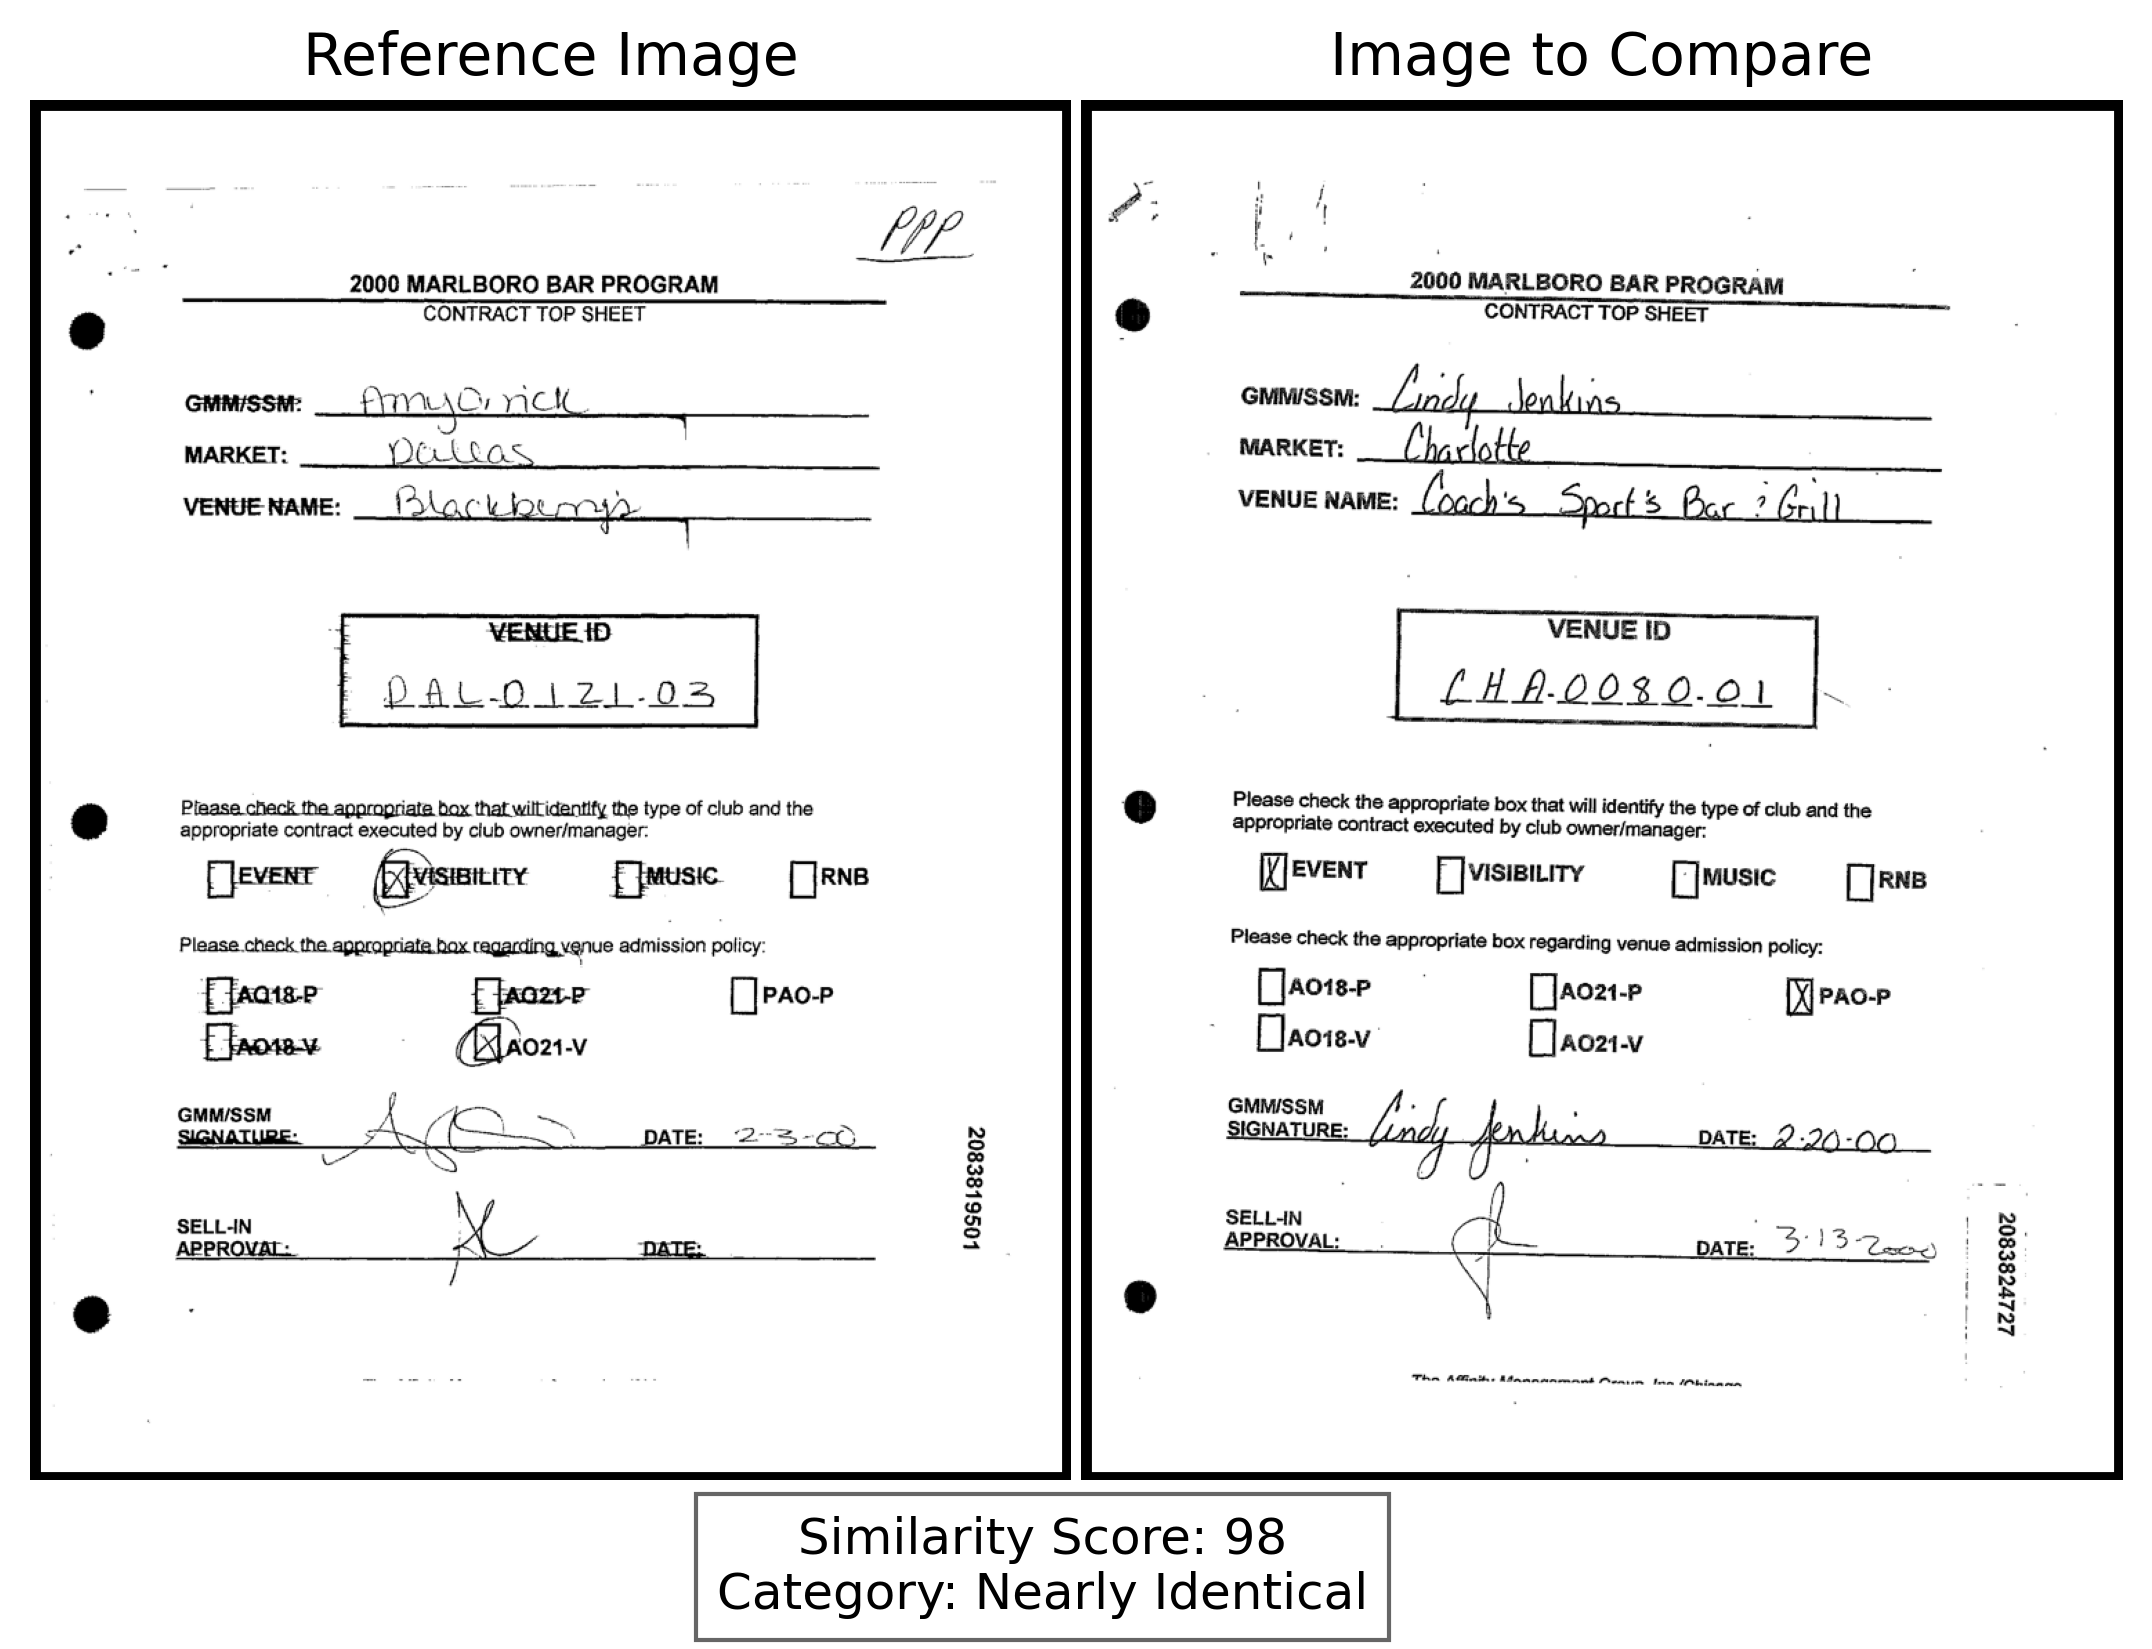
\includegraphics[width=\textwidth]{images/similar.png}
\vspace{0.2cm}
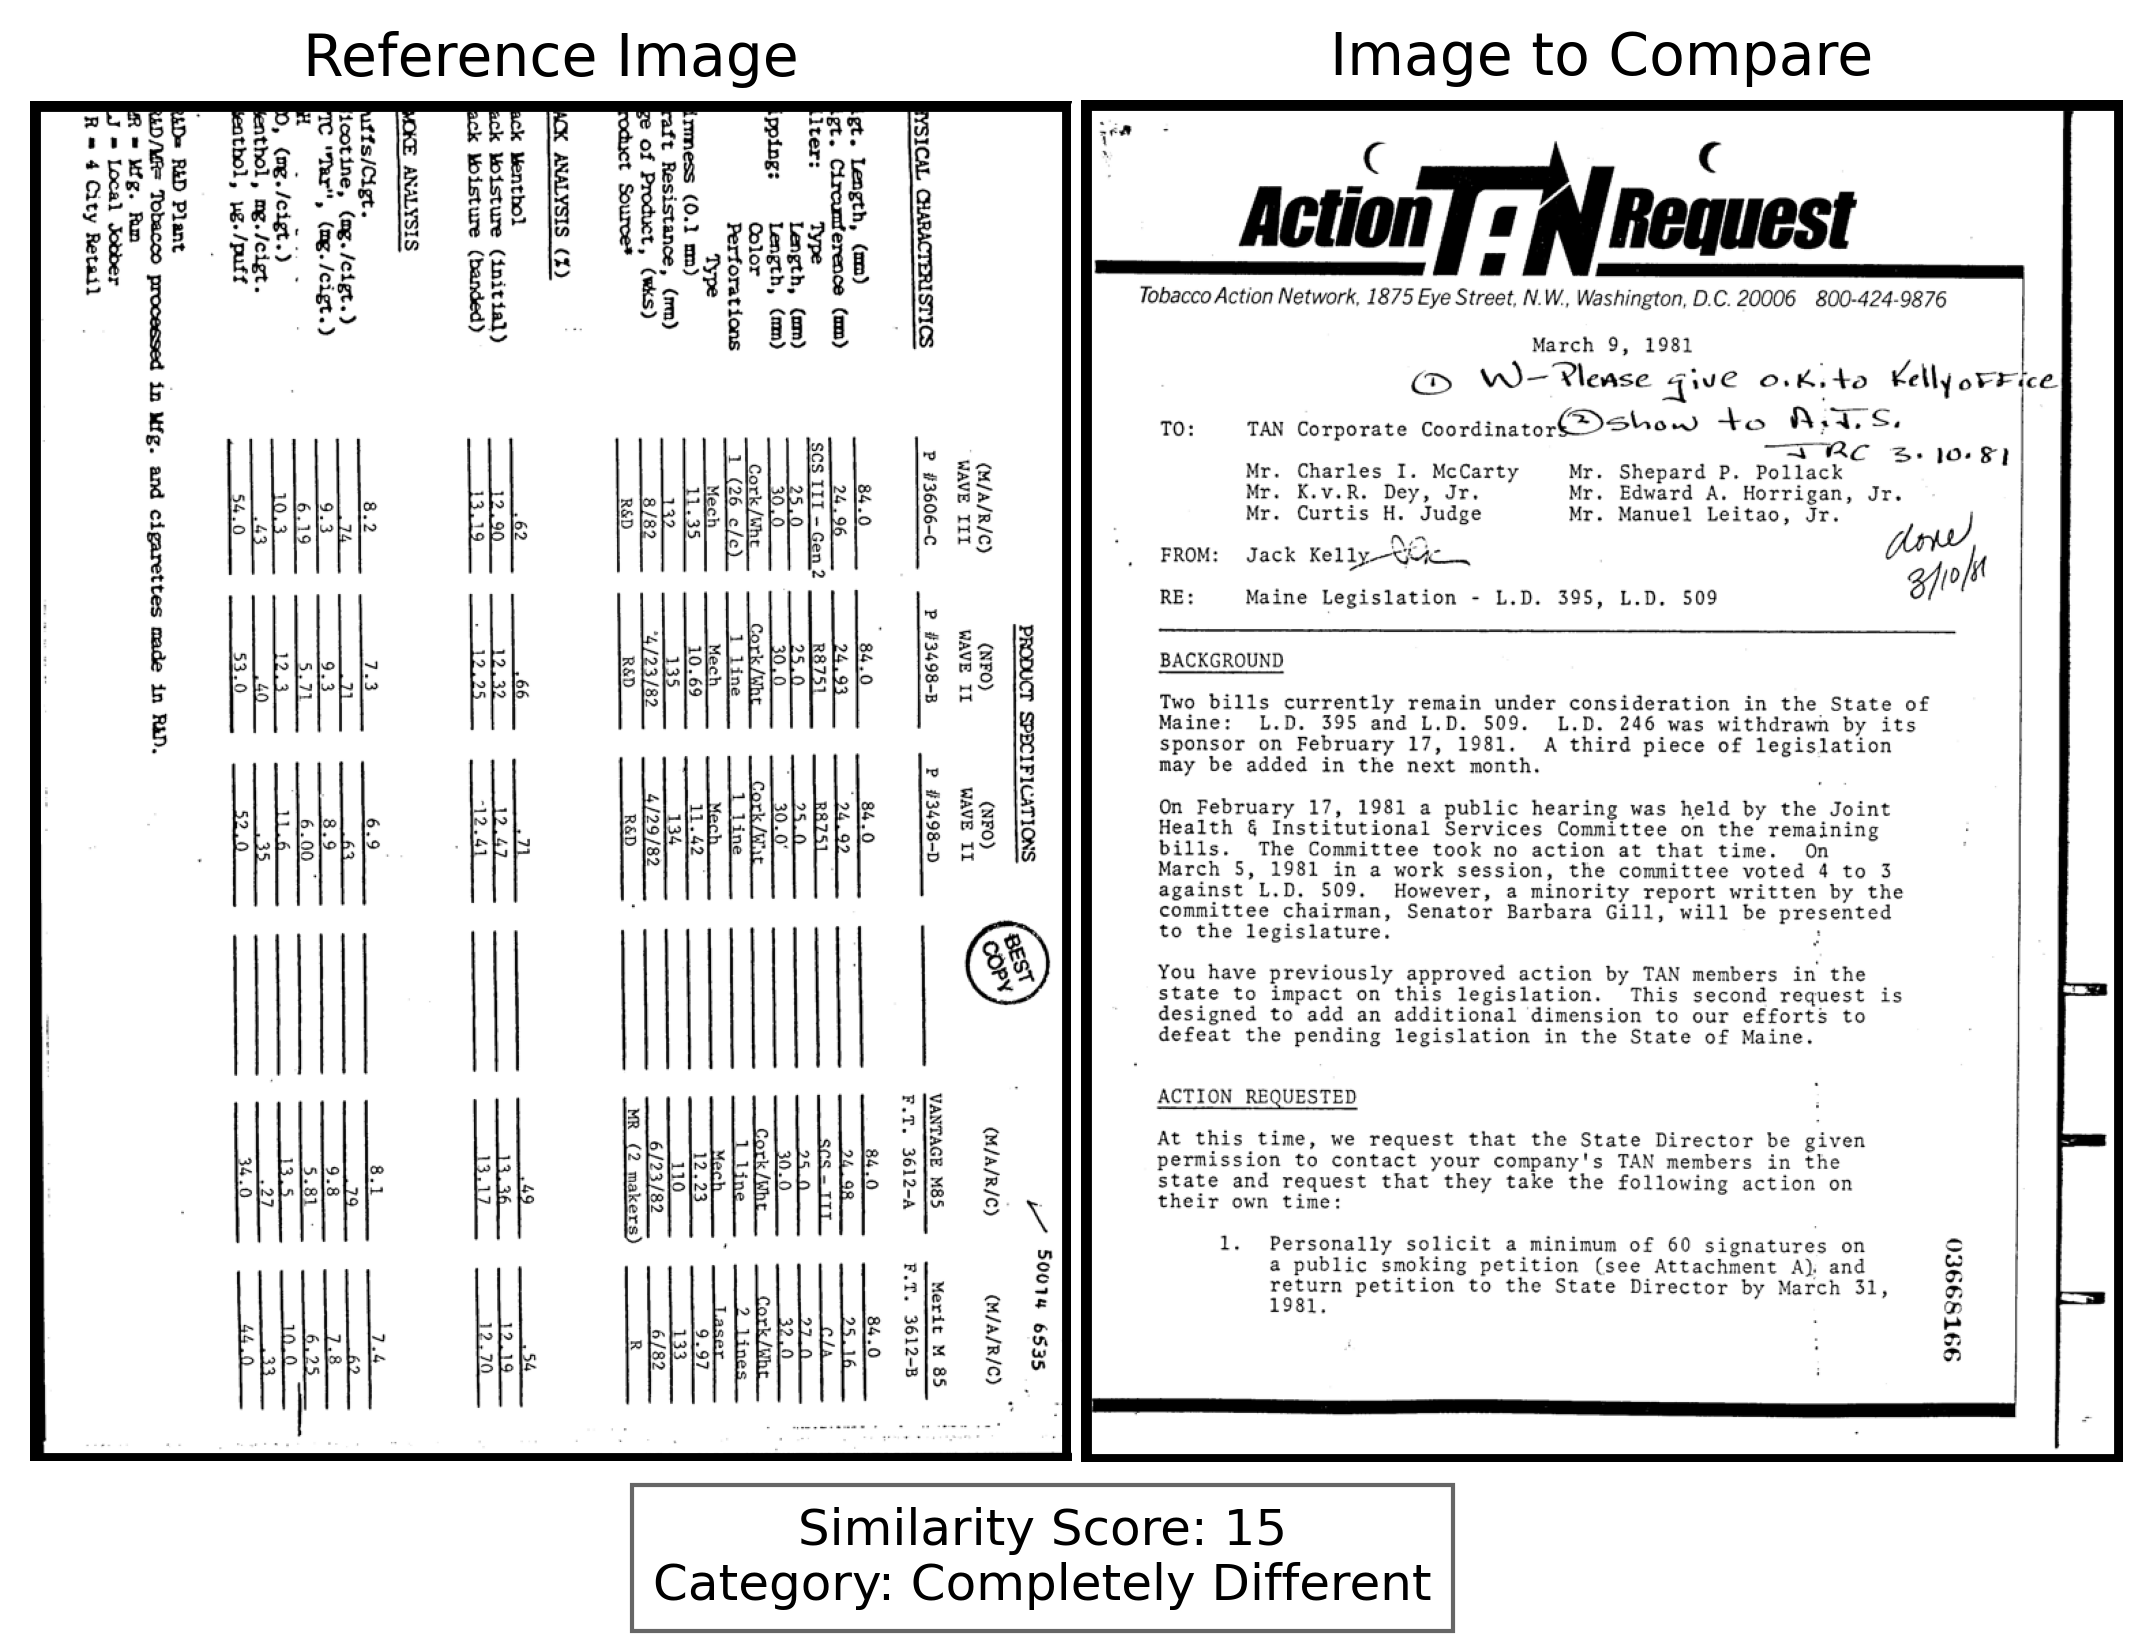
\includegraphics[width=\textwidth]{images/different.png}
\end{columns}
\end{frame}
